\section{Date: 2026-10-09}
\noindent \textbf{Series ID: EBZOXSLNQ} 

\noindent This series is titled Percent of Value of Loans, Small Business Administration (SBA) Backed for Zero Interval, Other Risk (Acceptable), Large Domestic Banks (DISCONTINUED) and has a frequency of Quarterly, 2nd Month's 1st Full Week. The units are Percent and the seasonal adjustment is Not Seasonally Adjusted.The observation start date is 2012-07-01 and the observation end date is 2017-04-01.The popularity of this series is 1. \\ 

\noindent \textbf{Series ID: EQTA25} 

\noindent This series is titled Total Equity to Total Assets, Banks with Total Assets from \$300M to \$1B, South Atlantic Census Division (DISCONTINUED) and has a frequency of Quarterly, End of Period. The units are Percent and the seasonal adjustment is Not Seasonally Adjusted.The observation start date is 1988-01-01 and the observation end date is 2020-07-01.The popularity of this series is 1. \\ 

\subsection{Raw Regression}
\noindent Regresses the two series against each other directly. A significant result here can come just as easily from both series sharing a long-run trend as from any real relationship.

\begin{center}
\begin{tabular}{lclc}
\toprule
\textbf{Dep. Variable:}         & value\_fred\_EQTA25 & \textbf{  R-squared:         } &     0.101   \\
\textbf{Model:}                 &         OLS         & \textbf{  Adj. R-squared:    } &     0.051   \\
\textbf{Method:}                &    Least Squares    & \textbf{  F-statistic:       } &     2.020   \\
\textbf{Date:}                  &   Fri, 09 Oct 2026  & \textbf{  Prob (F-statistic):} &    0.172    \\
\textbf{Time:}                  &       17:37:27      & \textbf{  Log-Likelihood:    } &   -1.8044   \\
\textbf{No. Observations:}      &            20       & \textbf{  AIC:               } &     7.609   \\
\textbf{Df Residuals:}          &            18       & \textbf{  BIC:               } &     9.600   \\
\textbf{Df Model:}              &             1       & \textbf{                     } &             \\
\textbf{Covariance Type:}       &      nonrobust      & \textbf{                     } &             \\
\bottomrule
\end{tabular}
\begin{tabular}{lcccccc}
                                & \textbf{coef} & \textbf{std err} & \textbf{t} & \textbf{P$> |$t$|$} & \textbf{[0.025} & \textbf{0.975]}  \\
\midrule
\textbf{const}                  &      10.3095  &        0.071     &   145.966  &         0.000        &       10.161    &       10.458     \\
\textbf{value\_fred\_EBZOXSLNQ} &      -0.0676  &        0.048     &    -1.421  &         0.172        &       -0.168    &        0.032     \\
\bottomrule
\end{tabular}
\begin{tabular}{lclc}
\textbf{Omnibus:}       &  4.776 & \textbf{  Durbin-Watson:     } &    0.282  \\
\textbf{Prob(Omnibus):} &  0.092 & \textbf{  Jarque-Bera (JB):  } &    2.226  \\
\textbf{Skew:}          & -0.525 & \textbf{  Prob(JB):          } &    0.329  \\
\textbf{Kurtosis:}      &  1.747 & \textbf{  Cond. No.          } &     1.92  \\
\bottomrule
\end{tabular}
%\caption{OLS Regression Results}
\end{center}

Notes: \newline
 [1] Standard Errors assume that the covariance matrix of the errors is correctly specified.

\begin{figure}
\centering
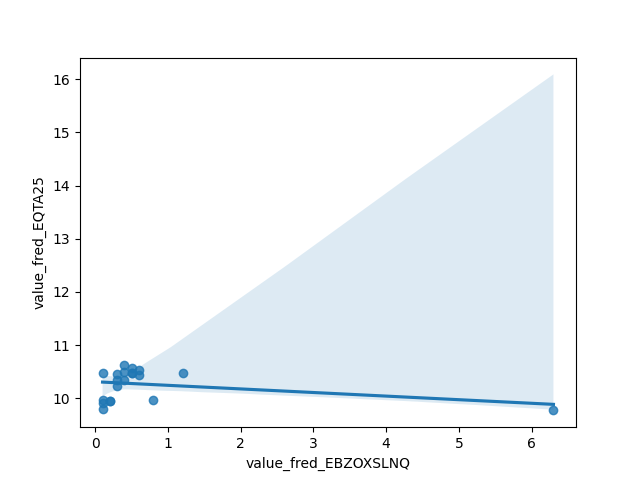
\includegraphics[scale = 0.9]{plots/plot_2026-10-09.png}
\caption{Raw Regression Plot for 2026-10-09}
\end{figure}
\newpage
\subsection{Detrended Regression}
\noindent Regresses the residuals of each series after removing its own linear time trend, so a shared trend can no longer drive the result on its own. A relationship that stays significant here is better evidence of a genuine link between the two series.

\begin{center}
\begin{tabular}{lclc}
\toprule
\textbf{Dep. Variable:}                    & value\_fred\_EQTA25\_detrended & \textbf{  R-squared:         } &     0.090   \\
\textbf{Model:}                            &              OLS               & \textbf{  Adj. R-squared:    } &     0.039   \\
\textbf{Method:}                           &         Least Squares          & \textbf{  F-statistic:       } &     1.777   \\
\textbf{Date:}                             &        Fri, 09 Oct 2026        & \textbf{  Prob (F-statistic):} &    0.199    \\
\textbf{Time:}                             &            17:37:27            & \textbf{  Log-Likelihood:    } &    9.0990   \\
\textbf{No. Observations:}                 &                 20             & \textbf{  AIC:               } &    -14.20   \\
\textbf{Df Residuals:}                     &                 18             & \textbf{  BIC:               } &    -12.21   \\
\textbf{Df Model:}                         &                  1             & \textbf{                     } &             \\
\textbf{Covariance Type:}                  &           nonrobust            & \textbf{                     } &             \\
\bottomrule
\end{tabular}
\begin{tabular}{lcccccc}
                                           & \textbf{coef} & \textbf{std err} & \textbf{t} & \textbf{P$> |$t$|$} & \textbf{[0.025} & \textbf{0.975]}  \\
\midrule
\textbf{const}                             &    6.819e-13  &        0.036     &  1.88e-11  &         1.000        &       -0.076    &        0.076     \\
\textbf{value\_fred\_EBZOXSLNQ\_detrended} &      -0.0374  &        0.028     &    -1.333  &         0.199        &       -0.096    &        0.022     \\
\bottomrule
\end{tabular}
\begin{tabular}{lclc}
\textbf{Omnibus:}       &  3.941 & \textbf{  Durbin-Watson:     } &    0.613  \\
\textbf{Prob(Omnibus):} &  0.139 & \textbf{  Jarque-Bera (JB):  } &    1.420  \\
\textbf{Skew:}          & -0.117 & \textbf{  Prob(JB):          } &    0.492  \\
\textbf{Kurtosis:}      &  1.716 & \textbf{  Cond. No.          } &     1.29  \\
\bottomrule
\end{tabular}
%\caption{OLS Regression Results}
\end{center}

Notes: \newline
 [1] Standard Errors assume that the covariance matrix of the errors is correctly specified.

\begin{figure}
\centering
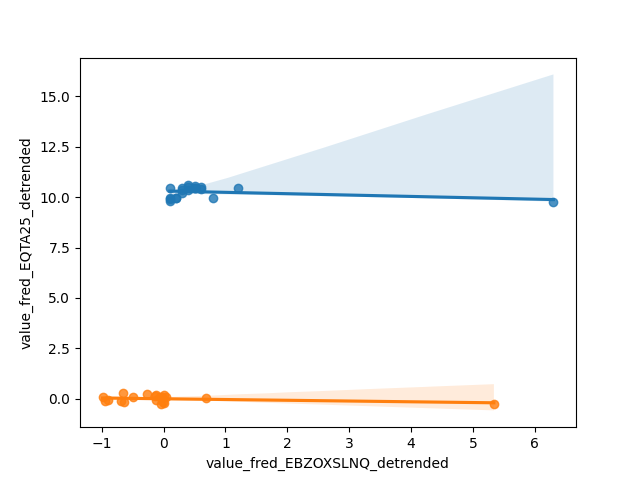
\includegraphics[scale = 0.9]{plots/plot_2026-10-09_detrended.png}
\caption{Detrended Regression Plot for 2026-10-09}
\end{figure}
\newpage
